\section{Generating the Data \label{sec:data}}

The raw data used in this project consist of simulated three-dimensional flight trajectories of launched spherical sports objects, such as tennis balls, baseballs, basketballs, or similar projectiles.
The goal of the simulation is not to model one specific ball type with maximal experimental accuracy, but rather to generate a broad and physically plausible family of trajectories that exhibit effects relevant for real ball flights: gravity, aerodynamic drag, wind, and spin-induced curvature due to the Magnus effect.\cite{mehta1985aerodynamics}\cite{goff2009trajectory}

For this purpose, $N=200000$ trajectories were generated, each resampled to $10000$ time points between launch and impact with the ground.
Each trajectory is represented by the time-dependent position
\begin{equation*}
    \vb{r}(t) = \begin{pmatrix}
        x(t) \\ y(t) \\ z(t)
    \end{pmatrix},
\end{equation*}
where $z=0$ denotes the ground plane.
The resulting dataset is therefore well suited for testing whether machine learning models can infer launch conditions or trajectory characteristics from complete, noisy, or partially observed flight paths.

\subsection{Physical Assumptions}

The projectile is modeled as a point mass moving in three spatial dimensions.
The height coordinate $z$ is measured relative to a flat ground plane, and the integration is stopped once the projectile reaches $z=0$ from above.
The gravitational acceleration is assumed to be constant and homogeneous,
\begin{equation*}
    \vb{g} = \begin{pmatrix}
        0 \\ 0 \\ -g
    \end{pmatrix},
    \qquad
    g = \SI{9.81}{\meter\per\second\squared}.
\end{equation*}

Furthermore, the wind velocity is assumed to be spatially and temporally constant during a single trajectory.
The aerodynamic parameters are also kept constant along the trajectory, meaning that effects such as changing drag coefficients, turbulent flow transitions, deformation of the ball, or changing spin rate are neglected.
The spin direction is represented by a fixed unit vector $\hat{\vb{\omega}}$, and spin dynamics such as precession or spin decay are not modeled explicitly.
These assumptions lead to a controlled but still non-trivial simulation setting: the generated trajectories remain interpretable from the perspective of classical mechanics, while also containing enough variation to form a challenging machine learning dataset.

\subsection{Equations of Motion}

The dynamical state of a projectile is given by its position $\vb{r}$ and velocity $\vb{v}$,
\begin{equation*}
    \vb{y}(t) = \begin{pmatrix}
        \vb{r}(t) \\ \vb{v}(t)
    \end{pmatrix} = \begin{pmatrix}
        x(t) \\ y(t) \\ z(t) \\ v_x(t) \\ v_y(t) \\ v_z(t)
    \end{pmatrix}.
\end{equation*}

The time evolution is determined by Newton's equation in first-order form,
\begin{equation*}
    \dv{\vb{r}}{t} = \vb{v}, \qquad \dv{\vb{v}}{t} = \vb{a}.
\end{equation*}

In addition to gravity, two aerodynamic forces are included: quadratic drag and a simplified Magnus acceleration.
Since aerodynamic forces depend on the velocity relative to the surrounding air, the relative velocity is defined as
\begin{equation*}
    \vb{q} = \vb{v} - \vb{u},
\end{equation*}
where $\vb{u}$ is the wind velocity.
The acceleration model used in the simulation is
\begin{equation}
  \dv{\vb{v}}{t} = \underbrace{
        \begin{pmatrix}
            0 \\ 0 \\ -g
        \end{pmatrix}
    }_{\text{gravity}}
    - \underbrace{
        \beta_D \norm{\vb{q}} \vb{q}
    }_{\text{drag}}
    + \underbrace{
        \beta_M \left( \hat{\vb{\omega}} \times \vb{q} \right)
    }_{\text{Magnus effect}}.
    \label{eq:eom}
\end{equation}
Here, $\beta_D$ is an effective drag parameter and $\beta_M$ is an effective Magnus parameter.
The drag term is opposite to the relative motion through the air and scales quadratically with the relative speed, since
\begin{equation*}
    \norm{\vb{q}} \vb{q}
\end{equation*}
has magnitude $\norm{\vb{q}}^2$.
The Magnus term acts perpendicular to both the spin axis and the relative velocity, producing curved trajectories for spinning balls.\cite{mehta1985aerodynamics}\cite{goff2009trajectory}
The parameters $\beta_D$ and $\beta_M$ absorb several physical constants, such as mass, radius, cross-sectional area, air density, drag coefficient, spin magnitude, and lift coefficient.
This is useful because the purpose of the simulation is to generate a diverse family of trajectories rather than to separately identify every microscopic physical parameter.

The initial position is chosen as
\begin{equation*}
    \vb{r}_0 = \begin{pmatrix}
        0 \\ 0 \\ \epsilon
    \end{pmatrix}, \qquad \epsilon = 10^{-6},
\end{equation*}
where the small offset $\epsilon$ prevents the event detection from immediately identifying the ball as being on the ground at $t=0$.
The initial velocity is parameterized using a speed $v_0$, a polar angle $\theta$, and an azimuthal angle $\phi$:
\begin{equation*}
    \vb{v}_0 = v_0 \begin{pmatrix}
        \sin\theta \cos\phi \\
        \sin\theta \sin\phi \\
        \cos\theta
    \end{pmatrix}.
\end{equation*}

In this convention, $\theta=0$ corresponds to a vertical launch and $\theta \approx \pi/2$ corresponds to an almost horizontal launch.
The ordinary differential equation in Eq. \eqref{eq:eom} is integrated numerically until the first downward crossing of the ground plane,
\begin{equation*}
    z(t_{\mathrm{hit}}) = 0, \qquad \dot{z}(t_{\mathrm{hit}}) < 0.
\end{equation*}
After integration, each trajectory is resampled to a fixed number of time points using the normalized time coordinate
\begin{equation*}
    \tau = \frac{t}{t_{\mathrm{hit}}} \in [0,1].
\end{equation*}
This ensures that all simulated examples have the same array shape, even though their physical flight times differ.

\subsection{Launch and Environmental Parameters}

Each trajectory is generated by randomly sampling a set of launch, aerodynamic, wind, and spin parameters.
The sampled parameter vector is
\begin{equation*}
    \vb{\lambda} = \left(
        v_0,
        \theta,
        \phi,
        u_x,
        u_y,
        u_z,
        \omega_x,
        \omega_y,
        \omega_z,
        \beta_D,
        \beta_M
    \right).
\end{equation*}

The wind vector is first sampled in spherical coordinates using a wind speed $u=\norm{\vb{u}}$, a polar angle $\theta_u$, and an azimuthal angle $\phi_u$, and is then converted to Cartesian components:
\begin{equation*}
    \vb{u} = u \begin{pmatrix}
        \sin\theta_u \cos\phi_u \\
        \sin\theta_u \sin\phi_u \\
        \cos\theta_u
    \end{pmatrix}.
\end{equation*}
Similarly, the spin direction is represented by a normalized vector
\begin{equation*}
    \hat{\vb{\omega}} = \begin{pmatrix}
        \omega_x \\ \omega_y \\ \omega_z
    \end{pmatrix}, \qquad \norm{\hat{\vb{\omega}}}=1.
\end{equation*}
Only the spin direction is sampled explicitly, while the magnitude of the spin contribution is absorbed into the effective coefficient $\beta_M$.
This reduces the number of independent degrees of freedom: instead of separately sampling spin magnitude, ball radius, mass, air density, and lift coefficient, the simulation uses the compact parameter $\beta_M$ to control the overall strength of the Magnus effect.
Analogously, $\beta_D$ controls the overall strength of air resistance.
This parameterization is advantageous for machine learning experiments because it keeps the input space lower-dimensional while still producing qualitatively realistic trajectory variations.

The default parameter ranges used in the dataset generation are summarized in Table~\ref{tab:simulation_ranges}.
The initial speed range $v_0 \in [0,\SI{75}{\meter\per\second}]$ was chosen to include a wide spectrum of sports-ball launch speeds, from very slow throws to high-speed shots or hits.
The launch direction is restricted to the upper hemisphere, $\theta \in [0,\pi/2)$, because downward initial launches are not considered in this dataset.
The azimuthal angle $\phi\in[0,2\pi)$ allows arbitrary horizontal launch directions.
The wind speed range $u\in[0,\SI{25}{\meter\per\second}]$ covers calm conditions as well as strong winds, while the wind direction is sampled over the full sphere.
Finally, the ranges of $\beta_D$ and $\beta_M$ were chosen broadly enough to produce trajectories ranging from nearly ballistic motion to strongly damped and noticeably curved flights.

\begin{table}[htbp]
    \centering
    \begin{tabular}{lll}
        \hline
        Parameter & Range & Physical meaning \\
        \hline
        $v_0$ & $[0, 75]\,\si{\meter\per\second}$ & Initial speed \\
        $\theta$ & $[0, \pi/2)$ & Launch polar angle \\
        $\phi$ & $[0, 2\pi)$ & Launch azimuthal angle \\
        $\beta_D$ & $[0.003, 0.04]\,\si{\per\meter}$ & Effective drag strength \\
        $\beta_M$ & $[0, 0.3]\,\si{\per\second}$ & Effective Magnus strength \\
        $u$ & $[0, 25]\,\si{\meter\per\second}$ & Wind speed \\
        $\theta_u$ & $[0, \pi]$ & Wind polar angle \\
        $\phi_u$ & $[0, 2\pi)$ & Wind azimuthal angle \\
        $\hat{\vb{\omega}}$ & $\norm{\hat{\vb{\omega}}}=1$ & Spin-axis direction \\
        \hline
    \end{tabular}
    \caption{Default parameter ranges used for trajectory generation. Angles are given in radians.}
    \label{tab:simulation_ranges}
\end{table}

The angular sampling is performed such that directions are distributed uniformly on the relevant sphere or hemisphere.
For example, instead of sampling the polar angle $\theta$ uniformly, the simulation samples $\cos\theta$ uniformly and then computes
\begin{equation*}
    \theta = \arccos(s),
\end{equation*}
where $s$ is uniformly distributed in the corresponding interval.
This avoids oversampling directions close to the polar axis, which would occur for naive uniform sampling of $\theta$.
The same idea is used for the wind direction over the full sphere.
The spin-axis direction $\hat{\vb{\omega}}$ is generated by drawing a three-dimensional Gaussian random vector and normalizing it to unit length, which also produces an isotropic distribution of directions.

\begin{figure}[htbp]
    \centering
    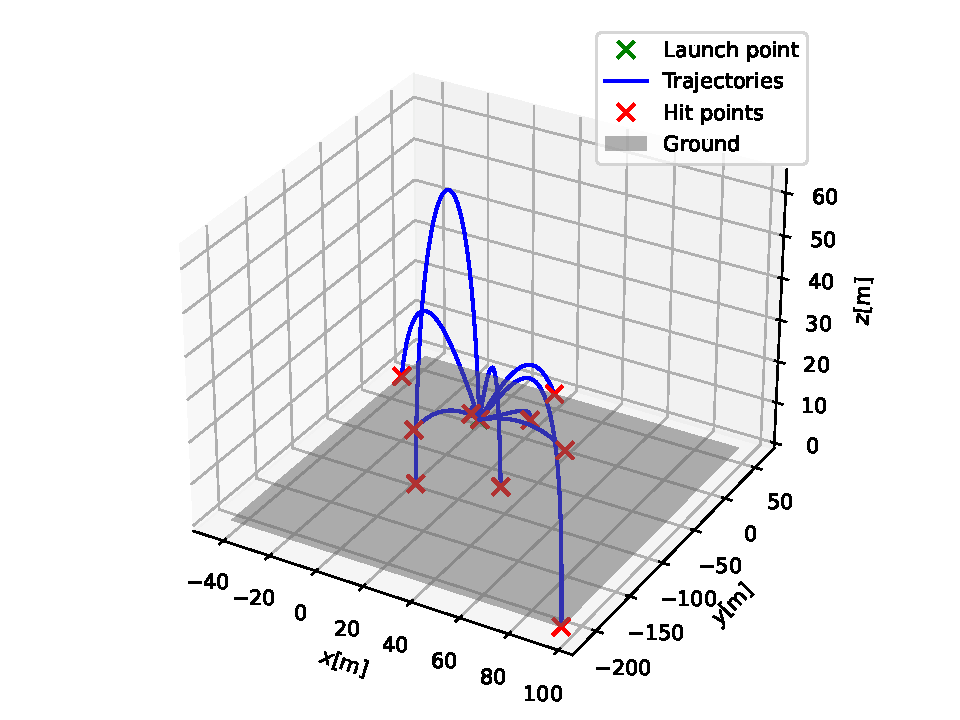
\includegraphics[width=\linewidth]{../figures/sample_trajectories_3d.pdf}
    \caption{Example 3D trajectories generated by the simulation. The curves illustrate the diversity of flight paths caused by different launch speeds, directions, drag strengths, wind vectors, and Magnus parameters.}
    \label{fig:sample_trajectories_3d}
\end{figure}

Overall, the simulation provides a controlled synthetic dataset with known physical parameters and tunable sources of trajectory variation.
This makes it possible to systematically study how different machine learning models behave when trained on full trajectories, engineered features, noisy observations, or cropped partial trajectories.
